\documentclass[a4paper]{article}

%% Language and font encodings
\usepackage[english]{babel}
\usepackage[utf8x]{inputenc}
\usepackage[T1]{fontenc}

%% Sets page size and margins
\usepackage[a4paper,top=3cm,bottom=2cm,left=3cm,right=3cm,marginparwidth=1.75cm]{geometry}

%% Useful packages
\usepackage{amsmath}
\usepackage{graphicx}
\usepackage[colorinlistoftodos]{todonotes}
\usepackage[colorlinks=true, allcolors=blue]{hyperref}

\title{Running Realtime Scheduling Analysis}
\author{Ilse Monserrat Sánchez Genereux and Mark Octavio Rivera Acosta}

\begin{document}
\maketitle

\begin{abstract}
The Linux kernel controls the way tasks (or processes) are managed in the running system. The task scheduler, sometimes called process scheduler, is the part of the kernel that decides which task to run next. In this project its analyzed the behavior of scheduler by changing a default value from the runtime scheduling. 
The default value is 950000µs, or 0.95 seconds for the sched\_rt\_runtime\_us or scheduler realtime running variable. Meaning that 5\% of the CPU time is reserved for processes that don't run under a real-time or deadline scheduling policy. This value in this file specifies how much of the "period" time can be used by all real-time and deadline scheduled processes on the system.
The AIO-Stress which shows the obtained results in the different tests is an a-synchronous I/O benchmark created by SuSE which is is a German Linux distribution provider and business unit of Novell, Inc.
\end{abstract}

\section{Introduction}

The Linux kernel controls the way tasks (or processes) are managed in the running system. The task scheduler, sometimes called process scheduler, is the part of the kernel that decides which task to run next. It is one of the core components of a multitasking operating system (such as Linux), being responsible for best utilizing system resources to guarantee that multiple tasks are being executed simultaneously. 

\setlength{\parskip}{3mm}

A typical real-time task is composed of a repetition of computation phases (task instances, or jobs) which are activated on a periodic or sporadic fashion.

\setlength{\parskip}{3mm}

The utilization of a real-time task is defined as the ratio between its WCET and its period (or minimum inter-arrival time), and represents the fraction of CPU time needed to execute the task.

\setlength{\parskip}{3mm}

In this project we will analyze the behavior of scheduler changing the default value of run time scheduling in terms of how many megabits per second change depending on how many microsecond are specified. 

\section{Theoretical Framework}

\subsection{The Kernel}
The kernel is the essential center of a computer operating system, the core that provides basic services for all other parts of the operating system. A synonym is nucleus. A kernel can be contrasted with a shell, the outermost part of an operating system that interacts with user commands. Kernel and shell are terms used more frequently in Unix operating systems than in IBM mainframe or Microsoft Windows systems.

\subsection{The Scheduler}
The scheduler is responsible for keeping the CPUs in the system busy. The Linux scheduler implements a number of scheduling policies, which determine when and for how long a thread runs on a particular CPU core.
Scheduling policies are divided into two major categories:

\begin{enumerate}

\item Realtime policies
\begin{itemize}
\item SCHED\_FIFO
\item SCHED\_RR
\end{itemize}
\item Normal Policies
\begin{itemize}
\item SCHED\_OTHER
\item SCHED\_BATCH
\item SCHED\_IDLE
\end{itemize}

\end{enumerate}

In this project we are dedicated to analyze the behavior of the Realtime policies by changing parameters in /proc/sys/kernel/sched\_rt\_period\_us which is described later.

\subsubsection{Realtime scheduling policies}

Realtime threads are scheduled first, and normal threads are scheduled after all realtime threads have been scheduled.
The realtime policies are used for time-critical tasks that must complete without interruptions.

\setlength{\parskip}{5mm}

\title{SCHED\_FIFO}

This policy is also referred to as static priority scheduling, because it defines a fixed priority (between 1 and 99) for each thread. The scheduler scans a list of SCHED\_FIFO threads in priority order and schedules the highest priority thread that is ready to run. This thread runs until it blocks, exits, or is preempted by a higher priority thread that is ready to run.
Even the lowest priority realtime thread will be scheduled ahead of any thread with a non-realtime policy; if only one realtime thread exists, the SCHED\_FIFO priority value does not matter.

\setlength{\parskip}{5mm}

In the Linux kernel, the SCHED\_FIFO policy includes a bandwidth cap mechanism. This protects realtime application programmers from realtime tasks that might monopolize the CPU. This mechanism can be adjusted through the following /proc file system parameters:

\setlength{\parskip}{5mm}

\begin{itemize}

\item \textbf{/proc/sys/kernel/sched\_rt\_period\_us}: Defines the time period to be considered one hundred percent of CPU bandwidth, in microseconds ('us' being the closest equivalent to 'µs' in plain text). The default value is 1000000µs, or 1 second.

\item \textbf{/proc/sys/kernel/sched\_rt\_runtime\_us}: Defines the time period to be devoted to running realtime threads, in microseconds ('us' being the closest equivalent to 'µs' in plain text). The default value is 950000µs, or 0.95 seconds.
\end{itemize}

\section {Objetives}
\begin{itemize}
\item Learn about Kernel scheduling, specifically running real time scheduling. 
\item Observe the change in AIO Stress when the microseconds increased. 
\end{itemize}

\section {Justification}
The need to learn about how the Linux kernel schedulers works, primarily to make an analysis of the changes to be made in the values of this. Also understand the meaning of the values that we will change and the relationship between the microseconds (run time) and the AIO Stress average.
 
\section {Development}
The default value is 950000µs, or 0.95 seconds for the sched\_rt\_runtime\_us or running realtime threads meaning that 5\% of the CPU time is reserved for processes that don't run under a real-time or deadline scheduling policy. This value in this file specifies how much of the "period" time can be used by all real-time and deadline scheduled processes on the system.  The value in this file can range from -1 to INT\_MAX-1.  Specifying -1 makes the run-time the same as the period; that is, no CPU time is set aside for non-real-time processes. 

Figure 1 shows the test results by changing the default value for this section of the scheduler. The microseconds µs were changed from 1,000,000 to 100,000 with a difference of 100,000 for each different test except by the default value. In this figure are included different parameters as Standard Error and Standard Deviation because the average AIO Stress can't be exact.
Figure 2 shows the relation between Microseconds and AIO Stress only. This shows how the results are varying going up and down.

\subsection{System Specifications}

This project was developed in a  DELL computer with the following specifications:

\begin{itemize}

\item Processor: Intel Core i7-4500U @ 3.00GHz (4 cores)
\item Motherboard: Dell 03VVKX
\item Chipset: Intel Haswell-UTL DRAM
\item Memory: 2 x 4096 MB DDR3-1600MHz
\item Disk: 1000GB Western Digital WD10JPVX-75J
\item Processor: Intel Core i7-4500U @ 3.00GHz (4 cores)
\item Audio:Intel Haswell-ULT HD Audio
\item Network: Realtek RTL8101/2/6E + Qualcomm Atheros QCA9565 / AR9565
\item OS: Ubuntu 16.04
\item Kernel:4.4.0-43-generic (x86\_64)
\item Desktop: Unity 7.4.0
\item Display Server: X Server 1.18.4
\item Display Driver: intel 2.99.917
\item OpenGL: 3.3 Mesa 11.2.0
\item Compiler: GCC 5.4.0 20160609
\item File-System: ext4
\item Screen Resolution: 1366x768

\end{itemize}

\begin{figure}
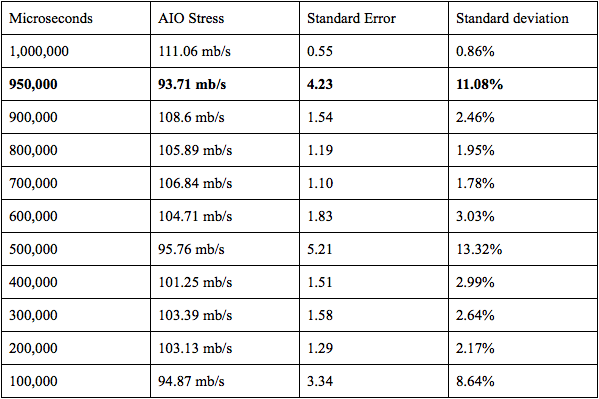
\includegraphics[width=1.0\textwidth]{Resultados.png}
\caption{\label{fig:Resultados} Results for the different test values}
\end{figure}

\begin{figure}
\centering
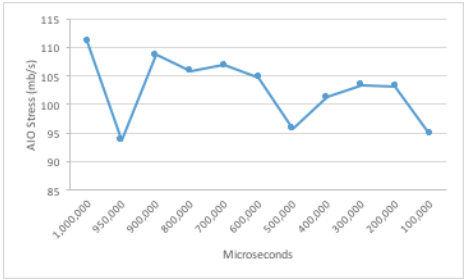
\includegraphics[width=1.0\textwidth]{Graph_Resultados.png}
\caption{\label{fig:Resultados Gráfica} Relation Microseconds-AIO Stress }
\end{figure}

\section {Conclusion}
The project was completed and thus further studies on the equipment, the use and importance of the scheduler in something so important to the computer as the kernel, although the kernel is the essential center of a computer operating system, the core that provides basic services for all other parts of the operating system, a kernel can be contrasted with a shell, the outermost part of an operating system that interacts with user commands. But what is noteworthy between these two is that the kernel has the scheduler, the unit responsible to keep busy the CPUs in the system, but this in a fully efficient manner. As seen throughout the development of this class, a scheduler may be a small part of the scheduler, but is very important because it coordinates the smooth operation between the processes occurring in the system, which operate the computer the way the user needs.

Importantly, the scheduler has within its configuration variables, which can be modified by a user in order to obtain an improvement in system performance and that was what was done in this project. It was learned to modify the scheduler to know and take notes on how to change the computer's performance and thus, together, find a specific value to achieve optimization of the computer.

It was very important practice because, although what was done can be found in books, is not the same know what can be done within a computer to really do it in practice and check for yourself how it changes so much with so little bit.

More importantly it was learned to appreciate what is the area of operating systems because if behind this project there was much research, imagine what must have researched and tested those who made the Linux OS.

\section {References}

	Kernel. (s.f.). Deadline Task Scheduling. Recovered by: https://www.kernel.org/doc/Documentation/scheduler/
    sched-deadline.txt

\setlength{\parskip}{3mm}

Open Suse.(s.f.). Tuning the time scheduler. Recovered by: https://doc.opensuse.org/documentation/html/
openSUSE\_121/opensuse-tuning/cha.tuning.taskscheduler.html

Phoronix Test Suite. (2016). OpenBenchmarking.org. Retrieved from AIO-Stress [pts/aio-stress] : https://openbenchmarking.org/test/pts/aio-stress

Red Hat. (s.f.). CPU Scheduling. Recovered by: https://access.redhat.com/documentation/en-US/Red\_Hat\_Enterprise\_Linux/6/html/Performance\_Tuning\_Guide/s-cpu-scheduler.html

\end{document}
